\chapter{Resumen de la Arquitectura del Código ESP32}

Este capítulo explica la arquitectura interna del repositorio \texttt{ESP32\_BT\_Controller} basándose en el diagrama al final de este capítulo.
Describe cómo la aplicación Android se comunica con el firmware del ESP32, cómo se decodifican los comandos de entrada,
y cómo esos comandos se convierten en salidas reales de hardware (motores, señales PWM, interruptores), con telemetría y funciones de depuración opcionales.

\section{Arquitectura de Alto Nivel (Android App \texorpdfstring{$\leftrightarrow$}{<->} ESP32)}

El sistema está construido alrededor de un enlace \textbf{Bluetooth SPP (Serial Port Profile)}:

\begin{itemize}
    \item La \textbf{Android App} envía dos tipos de paquetes:
    \begin{itemize}
        \item \textbf{Paquetes de Estado RC} (estado de control continuo: joysticks, perillas, máscara de bits de interruptores).
        \item \textbf{Paquetes de Evento} (eventos de pulsación de botones que disparan pulsos cortos).
    \end{itemize}
    \item El \textbf{firmware del ESP32} recibe estos paquetes, actualiza estructuras de datos compartidas, y aplica continuamente el
    estado de control más reciente a las salidas de hardware.
    \item Opcionalmente, el ESP32 envía \textbf{paquetes de telemetría} de vuelta a la aplicación Android (datos de panel/indicador/gráfica y un mensaje de configuración de una sola vez).
\end{itemize}

\section{Capa de Inicialización (Diagrama: \textit{Initialization})}

Al inicio, \texttt{ESP32\_BT\_Controller.ino} ejecuta \texttt{setup()}, que llama a \texttt{systemInit()}.
Esta secuencia de arranque prepara las comunicaciones y el hardware.

\subsection{Inicialización Serial (\texttt{serialInit()})}
El firmware inicia el puerto serial USB a \texttt{115200} baudios.
Esto se usa principalmente para diagnósticos de desarrollo (impresiones de depuración), y no afecta directamente el control por Bluetooth.

\subsection{Inicialización Bluetooth (\texttt{bluetoothInit()})}
Bluetooth SPP se inicializa con:
\begin{itemize}
    \item \verb|SerialBT.begin("ESP32-BT")|
\end{itemize}
Esto crea el nombre del dispositivo con el que la aplicación se empareja y se conecta.

\subsection{Inicialización de Hardware (\texttt{hardwareInit()})}
La configuración de hardware está dividida en módulos para mantener el proyecto mantenible:

\begin{itemize}
    \item \texttt{boardInit()} --- configuración a nivel de placa (modos GPIO, valores por defecto de la placa).
    \item \texttt{i2cBusInit()} --- prepara el bus I\textsuperscript{2}C (si se usa).
    \item \texttt{halOutputsInit()} --- prepara los canales de salida PWM (LEDC) y los pines de salida.
    \item Opcional: \texttt{mcpInit()} --- inicializa un expansor de E/S MCP23017 si está habilitado.
    \item Opcional: \texttt{i2cSensorsInit()} --- inicializa sensores externos en I\textsuperscript{2}C si está habilitado.
\end{itemize}

\section{Capa de Ejecución (Diagrama: \textit{Runtime / main loop})}

Después de la inicialización, la función Arduino \texttt{loop()} se ejecuta continuamente.
En este repositorio:
\begin{itemize}
    \item \texttt{loop()} llama a \texttt{systemLoop()} (procesamiento central de control).
    \item \texttt{loop()} también llama a \texttt{pulseUpdate()} para salidas momentáneas.
\end{itemize}

Dentro de \texttt{systemLoop()}, el flujo principal de ejecución es:

\begin{enumerate}
    \item \textbf{Recibir y decodificar comandos Bluetooth} (\texttt{handleBluetooth()}).
    \item \textbf{Enviar telemetría cuando corresponda} (\texttt{sendTelemetryIfDue()}), solo cuando una aplicación está conectada.
    \item \textbf{Aplicar salidas de control} (\texttt{controlUpdate()}).
    \item \textbf{Impresión de depuración opcional} (controlada por \texttt{debug\_config.h}).
\end{enumerate}

\section{Subsistema de Recepción Bluetooth (Diagrama: \textit{Bluetooth RX (receiver)})}

El módulo receptor Bluetooth (\texttt{receiver.cpp}) es responsable de manejar el flujo de bytes crudo.
Debido a que los datos Bluetooth pueden llegar fragmentados o consecutivos, el receptor usa un enfoque de \textbf{buffer rodante}:

\begin{itemize}
    \item Leer bytes desde \texttt{SerialBT}.
    \item Buscar cabeceras de paquete válidas.
    \item Esperar hasta que la longitud completa del paquete esté presente.
    \item Copiar el paquete a una estructura de paquete compartida.
\end{itemize}

\subsection{Paquetes de Entrada}
El repositorio define formatos de paquetes fijos en \texttt{packets.h}:

\begin{description}
    \item[Paquete de Estado RC (\texttt{RcPacket})] Una instantánea continua de valores de control (joysticks, perillas, interruptores).
    Esta es la entrada principal para el control de motor/servo/PWM.
    \item[Paquete de Evento (\texttt{EventPacket})] Un paquete corto que contiene un \texttt{eventId}.
    Cuando se recibe, el firmware dispara un manejador de eventos para generar una acción de pulso.
\end{description}

\section{Modelo de Datos Compartido (Diagrama: \textit{packets.h})}

El archivo \texttt{packets.h} es la definición central de todos los formatos de mensajes usados en el sistema.
Es importante arquitectónicamente porque actúa como el contrato compartido entre módulos:

\begin{itemize}
    \item El receptor escribe el estado/evento decodificado más reciente en instancias globales de paquetes.
    \item La capa de control lee esas instancias de paquetes en cada iteración del bucle.
    \item La capa de telemetría crea paquetes salientes usando diseños fijos y sumas de verificación.
\end{itemize}

Esta separación hace que el sistema sea más fácil de extender: añadir un campo de telemetría o un nuevo tipo de paquete se hace de forma centralizada.

\section{Capa de Control (Diagrama: \textit{Control layer})}

La capa de control (\texttt{control.cpp}) convierte el estado RC recibido más recientemente en acciones de hardware:

\begin{itemize}
    \item Lee valores de joystick/perilla/interruptor del paquete de estado actual.
    \item Mapea rangos de control a rangos PWM.
    \item Llama funciones de salida HAL tales como:
    \begin{itemize}
        \item salida PWM de dirección,
        \item velocidad y dirección del motor,
        \item PWM de paneo de cámara,
        \item brillo de LED,
        \item intensidad del buzzer,
        \item salidas de interruptores.
    \end{itemize}
\end{itemize}

\subsection{Manejo de Eventos}
Cuando llega un \texttt{EventPacket}, el receptor dispara \texttt{controlHandleEvent(eventId)}.
Este manejador de eventos mapea un \texttt{eventId} a una acción de pulso corta (por ejemplo: pulsar un interruptor de salida específico).

\section{Capa de Abstracción de Hardware (Diagrama: \textit{HAL outputs})}

El módulo de salida HAL (\texttt{hal\_output.cpp}) es responsable de las operaciones de hardware de bajo nivel:

\begin{itemize}
    \item Generación PWM usando LEDC del ESP32 para servos, motores, brillo de LED e intensidad del buzzer.
    \item Control de dirección del motor usando pines GPIO dedicados de dirección.
    \item Rampa del motor usando una interrupción de temporizador para suavizar aceleración/desaceleración.
    \item Salidas de interruptores accionadas ya sea:
    \begin{itemize}
        \item directamente por pines GPIO del ESP32, o
        \item mediante el expansor MCP23017 opcional.
    \end{itemize}
\end{itemize}

\section{Expansión GPIO Opcional (Diagrama: \textit{MCP23017 (optional)})}

Si está habilitado, el MCP23017 proporciona líneas extra de E/S sobre I\textsuperscript{2}C.
El módulo \texttt{mcp\_io.cpp} maneja:

\begin{itemize}
    \item Escritura en registros del MCP para controlar salidas.
    \item Lectura de entradas desde el Puerto A del MCP (comúnmente usado para indicadores).
    \item Escritura de salidas en el Puerto B del MCP (comúnmente usado para interruptores/eventos).
\end{itemize}

\section{Subsistema de Telemetría (Diagrama: \textit{Telemetry TX} y \textit{Telemetry sources})}

El subsistema de telemetría (\texttt{telemetry.cpp}) envía datos de vuelta a la aplicación Android, pero solo cuando un cliente está conectado
(\texttt{SerialBT.hasClient()}).

\subsection{Comportamiento Consciente de la Conexión}
\begin{itemize}
    \item Si no hay un teléfono conectado, la telemetría no hace nada y reinicia su estado de ``configuración enviada''.
    \item Cuando un teléfono se conecta, el ESP32 primero envía un \textbf{mensaje de telemetría de configuración} de una sola vez
    (etiquetas para gráficas/paneles/indicadores) para que la aplicación pueda completar su interfaz.
    \item Después de eso, envía paquetes de telemetría periódicamente según intervalos de tiempo.
\end{itemize}

\subsection{Fuentes de Telemetría}
Los valores de telemetría son producidos por funciones fuente separadas (mostradas como \textit{Telemetry sources} en el diagrama),
por ejemplo lecturas ADC, máscaras digitales y valores de sensores opcionales.
El módulo de telemetría se enfoca en la construcción de paquetes y la planificación, no en decidir cómo se recogen los datos crudos.

\section{Subsistema de Depuración (Diagrama: \textit{Debug})}

El subsistema de depuración (\texttt{debug.cpp}) solo formatea e imprime información a \texttt{Serial}.
Está controlado por banderas de compilación en \texttt{debug\_config.h}:

\begin{itemize}
    \item las impresiones de joystick, perilla, interruptor y evento pueden habilitarse/deshabilitarse.
    \item la depuración no implementa lógica Bluetooth ni buffering de memoria; está separada intencionalmente.
\end{itemize}

\section{Subsistema de Pulsos (Diagrama: \textit{Pulse outputs})}

Algunas acciones del usuario son momentáneas (una pulsación de botón debería crear un pulso corto).
Este repositorio maneja ese comportamiento en el subsistema de pulsos:

\begin{itemize}
    \item \texttt{pulseUpdate()} se llama en el \texttt{loop()} de Arduino.
\end{itemize}

Esto mantiene la ``temporización de pulsos'' separada de la actualización principal de control y evita que las salidas se queden encendidas involuntariamente.

\section{Resumen: Por qué la Arquitectura está Estructurada de esta Manera}
El repositorio está organizado como una tubería de módulos especializados:

\begin{itemize}
    \item \textbf{Receiver} aísla la decodificación del flujo de bytes Bluetooth.
    \item \textbf{Packets} define el contrato de comunicación compartido.
    \item \textbf{Control} mapea entradas de la aplicación en acciones.
    \item \textbf{HAL} realiza escrituras de salida específicas de hardware.
    \item \textbf{Telemetry} maneja la planificación y el reporte de salidas.
    \item \textbf{Debug} proporciona visibilidad sin contaminar el código de lógica.
\end{itemize}

Esta separación hace que el firmware sea más fácil de mantener y extender (nuevas salidas, nuevos campos de telemetría, nuevos sensores),
mientras mantiene estable la comunicación con la aplicación Android.


%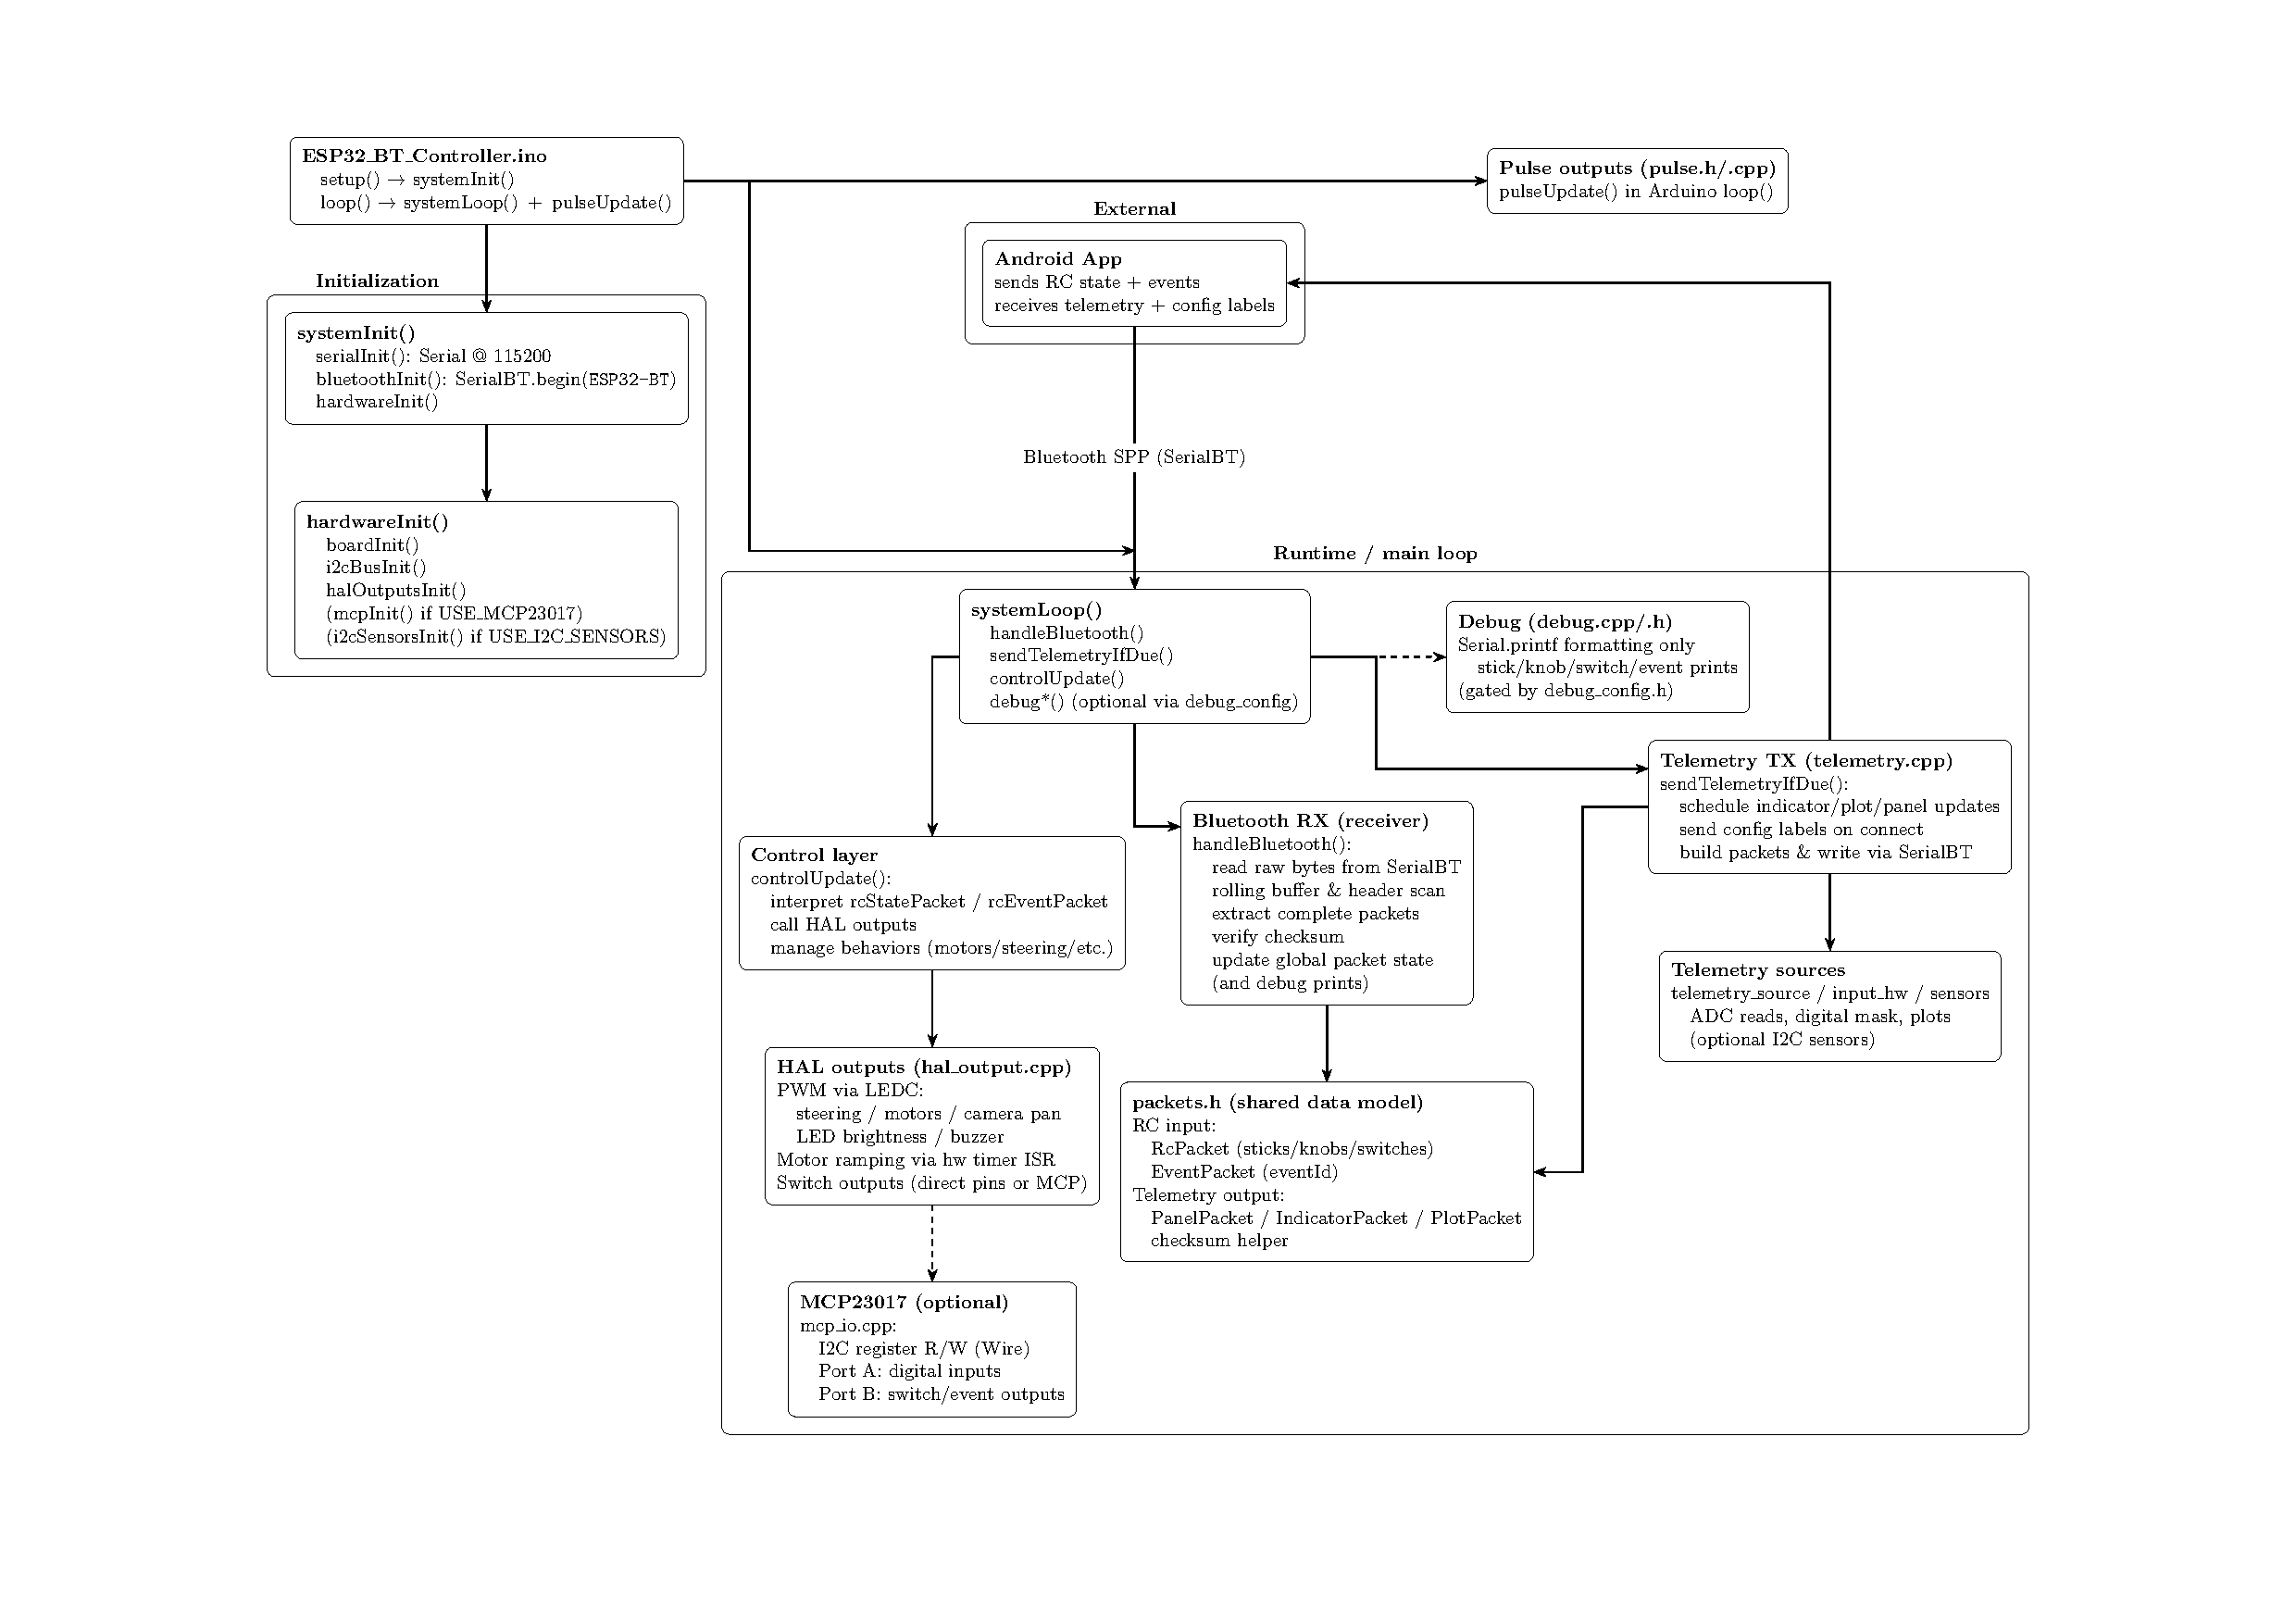
\includepdf[
%pages=1,
%landscape,
%fitpaper=false,
%pagecommand={
    %    \thispagestyle{plain}
    %    \begin{center}
        %        \vspace*{\fill}
        %        \rotatebox{90}{
            %            \parbox{0.7\textheight}{
                %                \centering
                %                \captionof{figure}{Arquitectura de software del ESP32.}
                %                \label{fig:esp32-arch}
                %            }
            %        }
        %    \end{center}
    %}
%]{Architecture_ESP32.pdf}




\includepdf[
pages=1,
landscape,
fitpaper=false,
offset=0 1cm,   % ← MOVER ARRIBA
pagecommand={
    \thispagestyle{plain}
    \begin{figure}[!b]
        \centering
        \caption{Arquitectura de software del ESP32.}
        \label{fig:esp32-arch}
    \end{figure}
}
]{Architecture_ESP32.pdf}



%\begin{landscape}
%    \begin{center}
    %        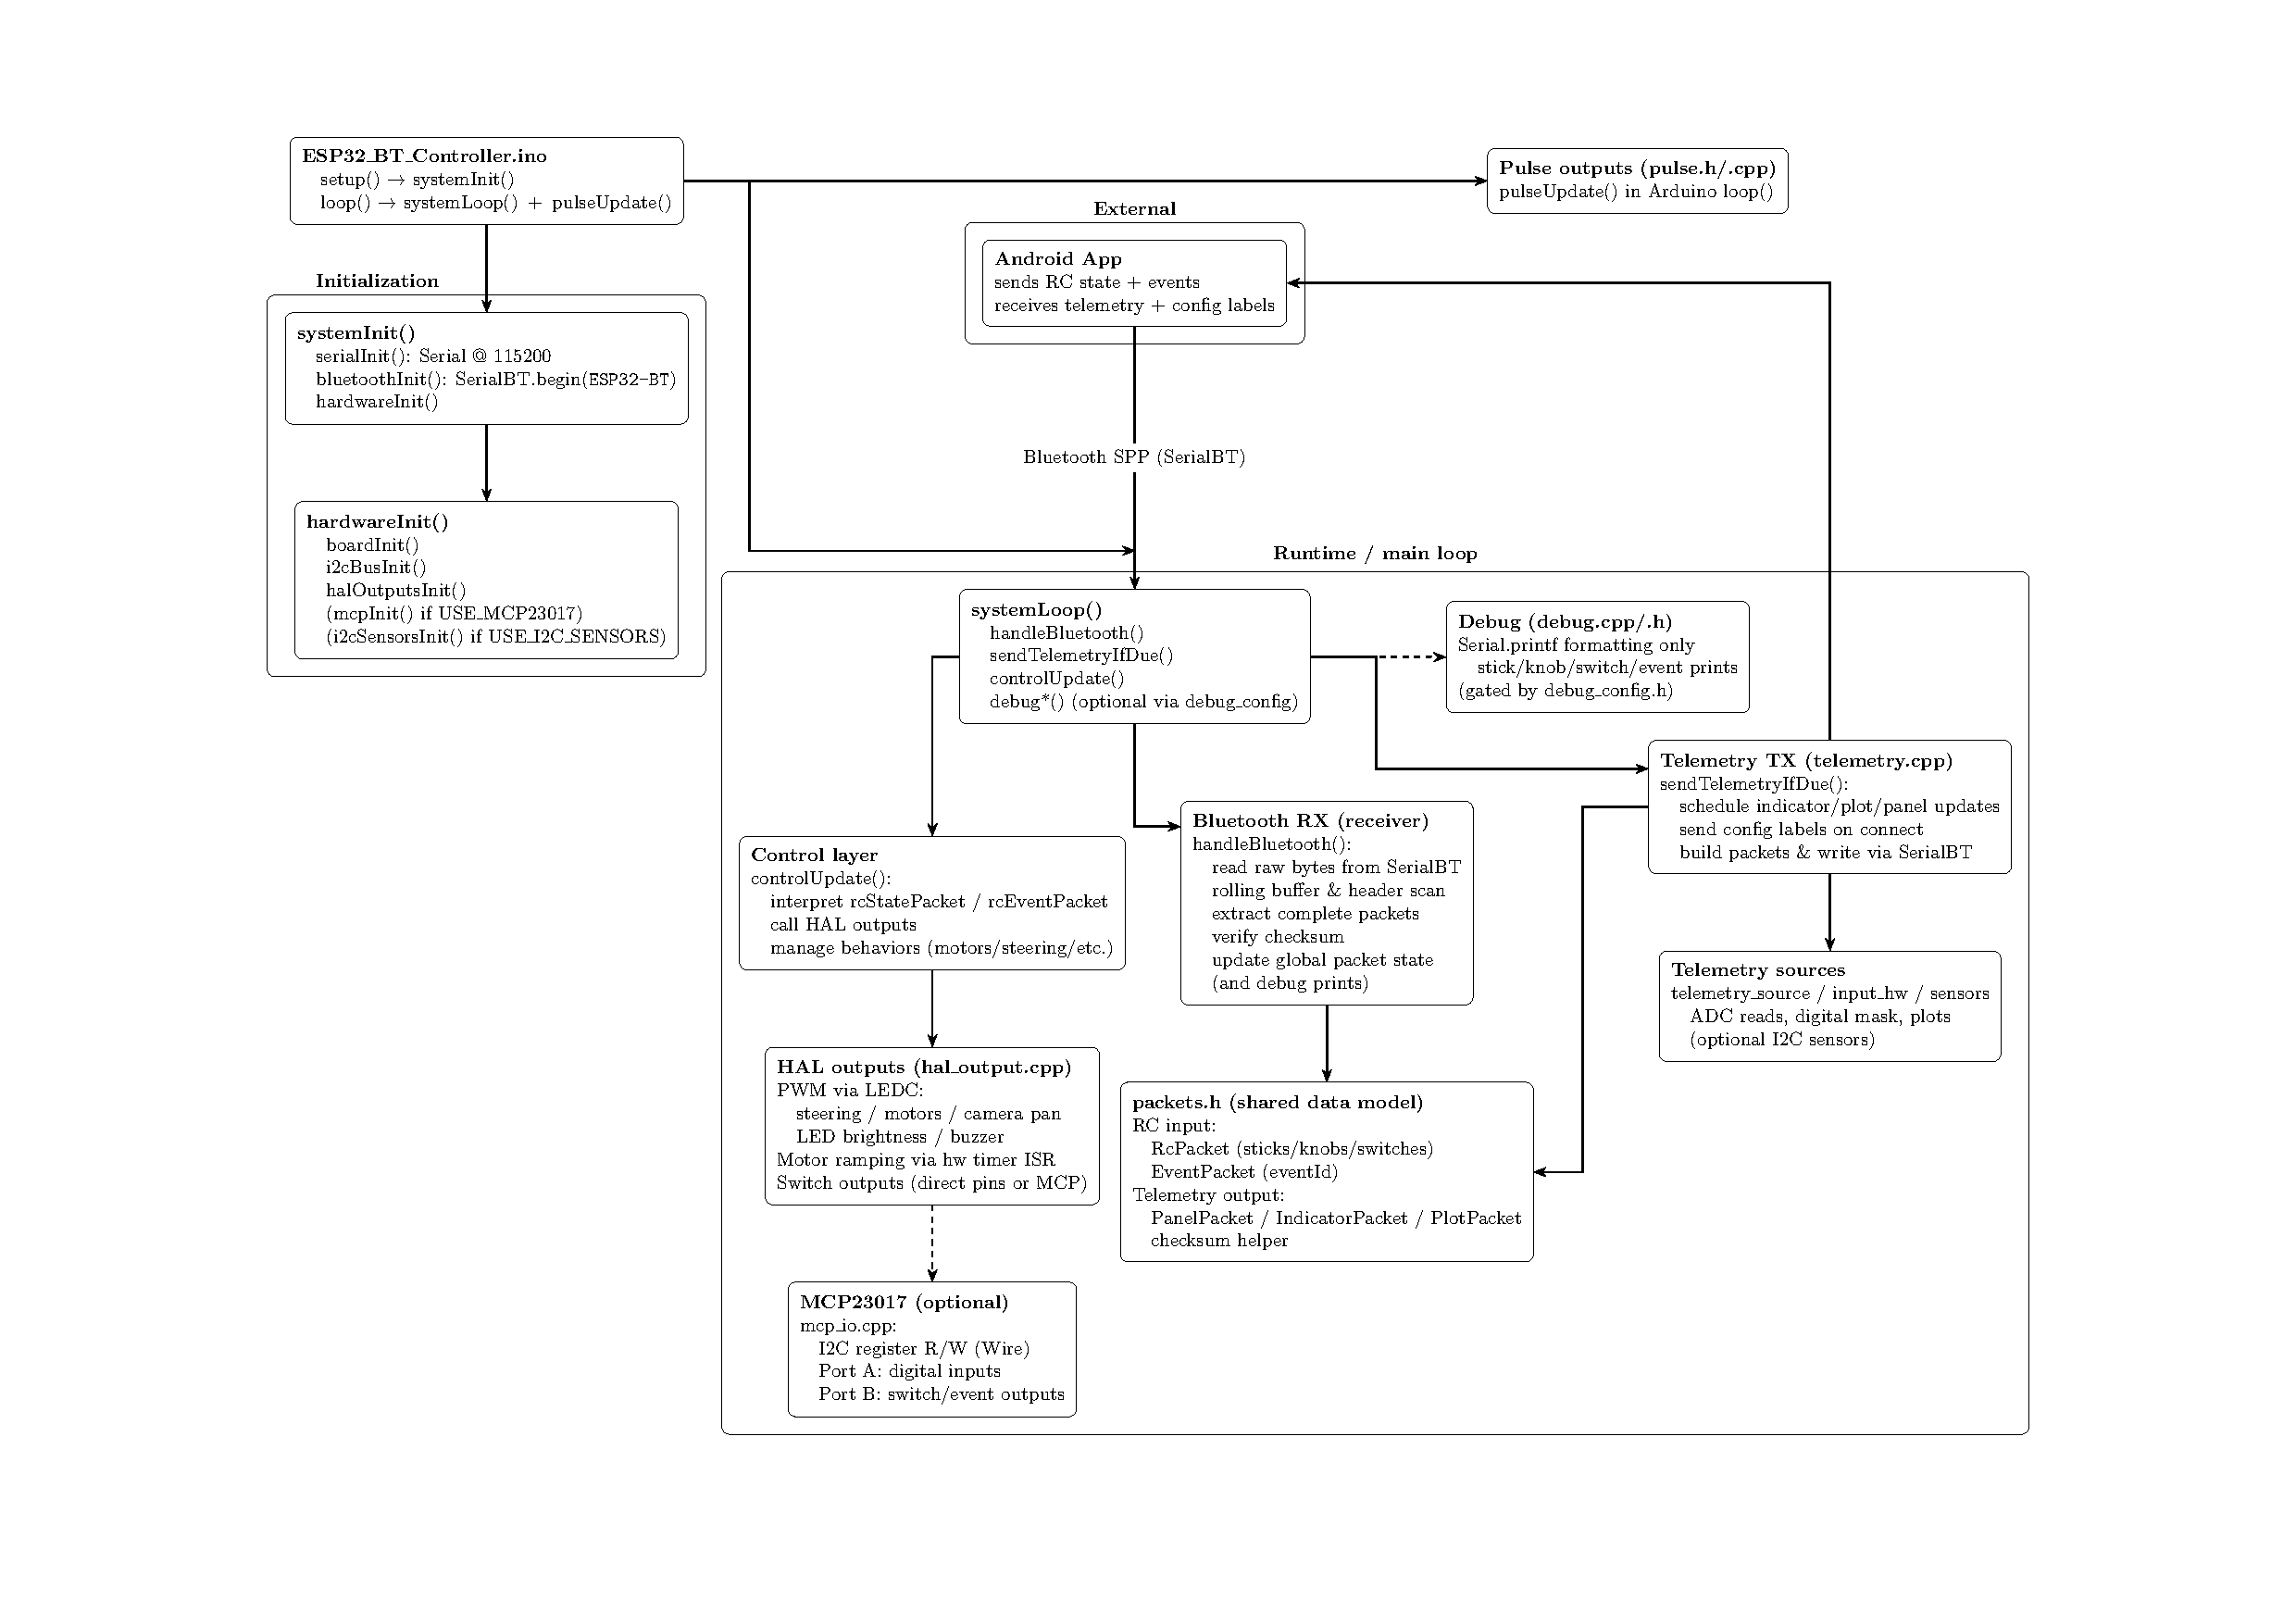
\includepdf[
    %        pages=1,
    %        landscape,
    %        fitpaper=false]{Architecture_ESP32.pdf}
    %    \end{center}
%\end{landscape}